\chapter{ESPECIFICAÇÕES FORMAIS}
	Neste capítulo são descritas as especificações formais da estrutura proposta. São descritos os requisitos funcionais e não funcionais buscados no desenvolvimento da aplicação, além das especificações do projeto por meio de diagrama de \textit{deployment}, diagramas de classe, diagrama de sequência e diagrama de atividades.
	
\section{Descrição da Aplicação}
	A aplicação proposta neste trabalho servirá apenas como exemplo para o objetivo principal que é o balanceamento de carga. A aplicação é consiste em um controle de finanças pessoais, com a possibilidade de registrar proventos e despesas. Para o balanceamento de carga será preparada uma estrutura utilizando \textit{containers}, separando em três camadas: persistência de dados, regra de negócio e interface \textit{web}.
	
\section{Requisitos}
	A seguir são apresentados os requisitos que devem ser atendidos pela aplicação desenvolvida. Os requisitos funcionais que devem ser atendidos pela aplicação desenvolvida são listados no Quadro \ref{Req-Func} e os não funcionais no Quadro \ref{Req-Nao-Func}
	
	\begin{table}[h]
		\caption{Requisitos Funcionais}
		\label{Req-Func}
		\begin{tabular}{|l|}
			\hline
			\textbf{REQUISITOS FUNCIONAIS} \\ \hline
			RF0: O sistema deve manter etiquetas \\ \hline
			RF1: O sistema deve manter transações \\ \hline
			RF2: O sistema deve manter períodos \\ \hline
			RF3: O sistema deve exibir o valor total de transações do período dividido entre proventos e despesas \\
			 \hline
	 		RF4: O sistema deve exibir o valor total das transações de cada etiqueta do período \\ \hline
			RF5: O sistema deve exibir com base nas transações o valor que há na carteira \\ \hline
			RF6: Transações com data futura não devem afetar o valor da carteira \\ \hline
		\end{tabular}
	\end{table}

	\begin{table}[!h]
		\caption{Requisitos Não Funcionais}
		\label{Req-Nao-Func}
		\begin{tabular}{|l|}
			\hline
			\textbf{REQUISITOS NÃO FUNCIONAIS} \\ \hline
			RNF0: O sistema deve estar no ar 24 horas por dia \\ \hline
			RNF1: O sistema deve separar interface, regras de negócio e persistência em \textit{containers} diferentes \\ \hline
			RNF2: O sistema deve aplicar balanceamento de carga \\ \hline
			RNF3: O sistema deve desenvolver as regras de negócio com a linguagem Java na versão 8\\ \hline
			RNF4: O sistema deve utilizar banco de dados PostgreSQL \\ \hline
			RNF5: O sistema deve utilizar \textit{containers} Docker \\ \hline
			RNF6: O sistema deve utilizar CORBA como \textit{middleware} \\ \hline
		\end{tabular}
	\end{table}

\section{Especificações}
	Nesta seção são apresentados os diagrama de \textit{deployment}, diagramas de classe, diagrama de sequência e diagrama de atividades, elaborados sob a Linguagem de Modelagem Unificada (\textit{Unified Modeling Language}, UML), para especificação do sistema proposto.
	
\subsection{Diagrama de \textit{Deployment}}
	No diagrama de \textit{deployment} apresentado na Figura \ref{Diagrama-Deployment} estão apresentados os componentes presentes na estrutura a ser desenvolvida.
	
	\begin{figure}[htb]
		\caption{Diagrama de \textit{Deployment}}
		{\parbox{6cm}{
				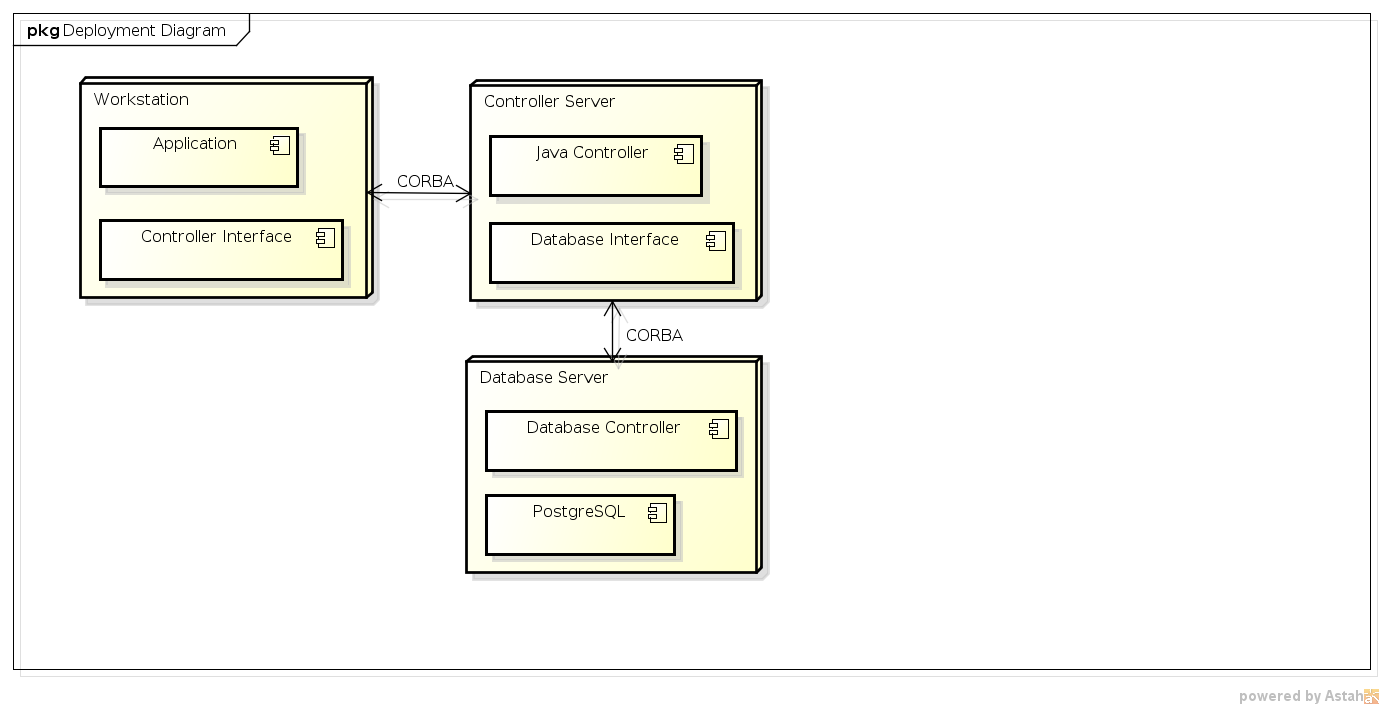
\includegraphics[width=14cm]{images/DeploymentDiagram.png}
				\label{Diagrama-Deployment}
				\fonte{Acervo do autor}
		}}
	\end{figure}

\subsection{Diagrama de Classe}
	As classes que compõem o sistema desenvolvido, bem como as relações entre cada classe, são apresentadas
	na Figura \ref{Diagrama-Classe} e servem também para a modelagem do \textit{middleware}.
	
	\begin{figure}[!htb]
		\caption{Diagrama de Classe}
		{\parbox{6cm}{
				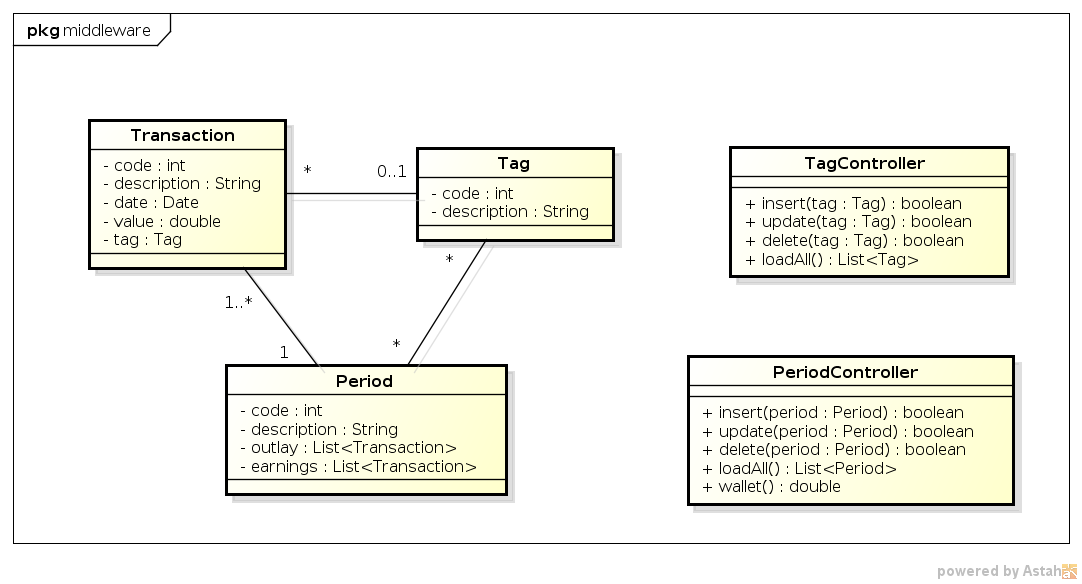
\includegraphics[width=10cm]{images/ClassDiagram.png}
				\label{Diagrama-Classe}
				\fonte{Acervo do autor}
		}}
	\end{figure}

\subsection{Diagramas de Sequência}
	Os diagramas de sequência das figuras \ref{SeqUser}, \ref{SeqSystem} e \ref{SeqQuestion} apresentam os fluxos básicos da aplicação.
	
	\begin{figure}[!htb]
		\caption{Diagrama de Sequência de adição de usuário}
		{\parbox{6cm}{
				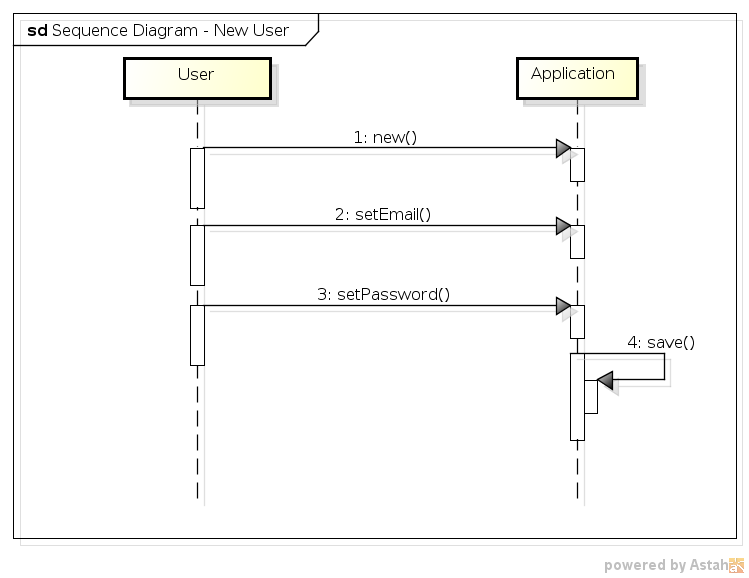
\includegraphics[width=10cm]{images/SequenceDiagramNewUser.png}
				\label{SeqUser}
				\fonte{Acervo do autor}
		}}
	\end{figure}

	\begin{figure}[!htb]
		\caption{Diagrama de Sequência de adição de Sistema}
		{\parbox{6cm}{
				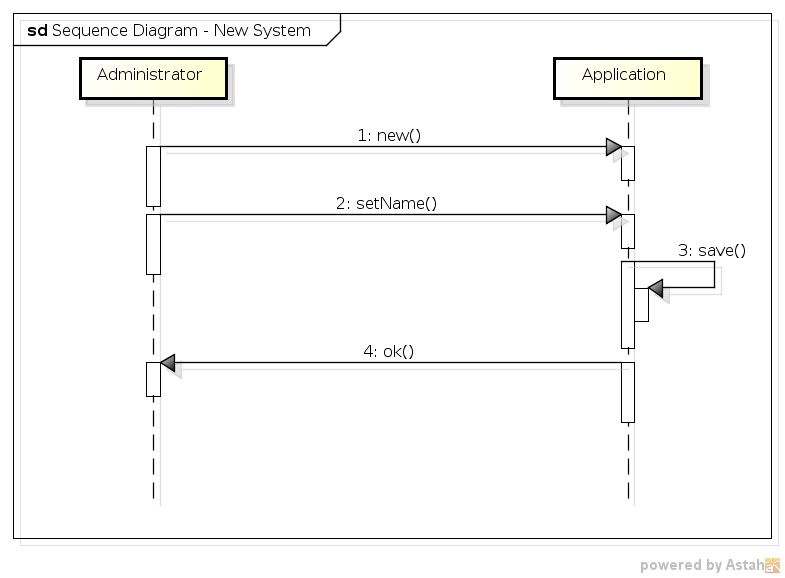
\includegraphics[width=10cm]{images/SequenceDiagramNewSystem.png}
				\label{SeqSystem}
				\fonte{Acervo do autor}
		}}
	\end{figure}

	\begin{figure}[!htb]
		\caption{Diagrama de Sequência de adição de pergunta}
		{\parbox{6cm}{
				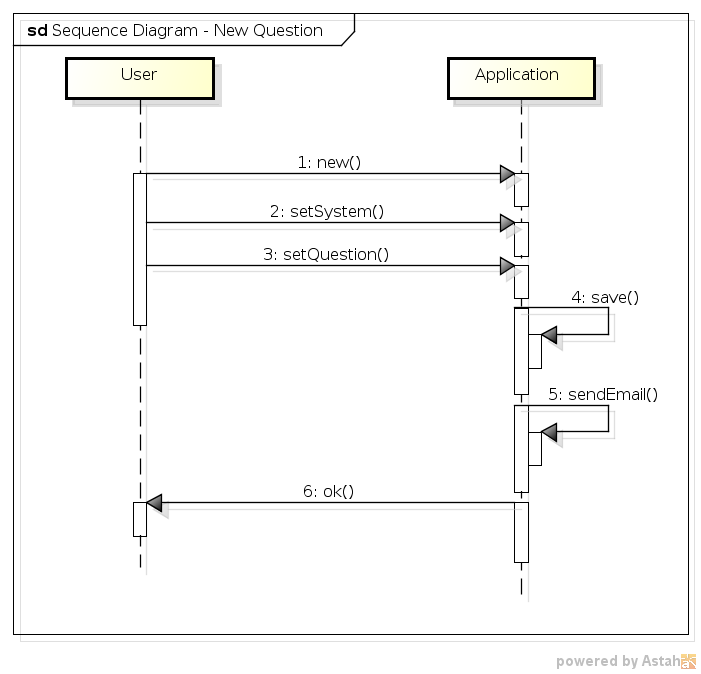
\includegraphics[width=10cm]{images/SequenceDiagramNewQuestion.png}
				\label{SeqQuestion}
				\fonte{Acervo do autor}
		}}
	\end{figure}